\documentclass[conference]{IEEEtran}
\IEEEoverridecommandlockouts

\usepackage{amsmath,amssymb}
\usepackage{graphicx}
\usepackage{booktabs,makecell}
\usepackage{xcolor}
\usepackage{cite}
\usepackage{xurl}
\usepackage{tikz}
\usetikzlibrary{positioning}
\usepackage[colorlinks=true,allcolors=blue]{hyperref}

% Placeholder for numbers that must come from the confirmed benchmark run.
% Every \tbd{} is replaced only after the engine results are final.
\newcommand{\tbd}[1]{\textcolor{red}{[TBD: #1]}}

\begin{document}

\title{Learner-State-Aware Generative User Interfaces:\\
A Closed-Loop Control Architecture for Adaptive Learning Environments}

\author{\IEEEauthorblockN{Omanand Prashant Swami, Sanjana Shashikant Chavan, K. V. Deshpande,\\
Pratik Rajendra Patil, Abhishek Ganesh Tirpude}
\IEEEauthorblockA{Dept. of Computer Science and Business Systems\\
JSPM's Rajarshi Shahu College of Engineering, Pune, India\\
\{opswami\_csbs, sschavan\_csbs, kvdeshpande\_comp, prpatil\_csbs, agtirpude\_csbs\}@jspmrscoe.edu.in}}

\maketitle

\begin{abstract}
Intelligent tutoring systems estimate what a learner knows but present a
fixed interface, while generative user interfaces (GenUI) synthesize
interfaces at runtime without any model of the learner. We propose a
closed-loop architecture that couples the two. Bayesian Knowledge Tracing
estimates mastery; a PID governor turns the mastery deficit into a structural
complexity budget; a rule-based policy selects scaffolding; a planner fixes the
layout closest to the budget; and a foundation model writes its content as a
JSON component tree, with a fallback when schema or budget checks fail. We evaluate the architecture in silico on
1,000 synthetic learners from three archetypes, replayed through four arms.
The closed loop keeps the rendered interface within 0.012 of the governor's
budget on average, against 0.131 for unconstrained GenUI and 0.123 for a
rule-based baseline, with 3.5 times less jitter than unconstrained GenUI,
which matches latent mastery slightly better but skips levels three times as
often. Standard BKT saturates after long success runs, so a later streak of
errors leaves the interface unchanged; a CUSUM lapse detector cuts overload
in a forgetting cohort by 25\%. In 300 single calls to the real model with the
planner (not full learner sessions), 98.7\% of raw outputs were within budget before any fallback, against 92\% when the model
also chose the layout. All claims concern algorithmic behavior;
no learning gains are claimed.
\end{abstract}

\begin{IEEEkeywords}
generative user interfaces, Bayesian knowledge tracing, PID control,
cognitive load, adaptive learning, simulation
\end{IEEEkeywords}

% ---------------------------------------------------------------------------
\section{Introduction}

Intelligent tutoring systems (ITS) have long modeled learners precisely.
Knowledge tracing maintains a probability that a learner has mastered each
knowledge component \cite{corbett1995knowledge}, and
tutors built on it have been deployed at scale in mathematics
\cite{ritter2007cognitive,vanlehn2011relative}. Their interface,
however, is authored in advance: the learner model selects the next problem,
not its presentation.

Generative user interfaces take the opposite position. A foundation model
produces a task-specific interface for each request
\cite{leviathan2026genui}, including interactive courseware
\cite{tu2026maicui}. These systems are open loop: the model does not observe
the learner's state, and nothing bounds how complex the generated interface
becomes.

Cognitive load theory explains why this matters. The same material can help
a novice and hinder an expert (the expertise reversal effect)
\cite{kalyuga2003expertise}, and guidance should fade as
competence grows \cite{renkl2003structuring,salden2010expertise}. An
adaptive interface therefore needs a learner model and a mechanism that holds
its complexity to that model without the abrupt changes that make adaptive
interfaces hard to use \cite{gajos2008predictability,findlater2004menus}.

BKT, PID control, layout search and constrained generation are each
established; our contribution is their integration: to our knowledge, the first
system in which a BKT mastery estimate, through feedback control, sets a
structural budget that a runtime-generated interface must meet:
\begin{enumerate}
\item A closed loop in which BKT mastery drives a PID governor whose
complexity budget is met by a layout planner and a generative model, with
schema validation and a fallback.
\item A computable structural complexity metric over a component tree for
linear-equation tasks, built from features linked to cognitive load.
\item An in-silico benchmark of 1,000 synthetic learners across four arms
and ablations, including an analysis of BKT saturation after success runs
and two remedies, with sensitivity analyses.
\end{enumerate}

% ---------------------------------------------------------------------------
\section{Related Work}

\paragraph*{Learner modeling}
Bayesian Knowledge Tracing (BKT) models each knowledge component as a
two-state hidden Markov model with prior, learning, guess and slip parameters
\cite{corbett1995knowledge}. Extensions individualize parameters
\cite{pardos2010individualization}, add forgetting \cite{khajah2016deep} or
contextualize guess and slip \cite{baker2008contextual}; its fixed points are
analyzed in \cite{vandesande2013properties}. Extended BKT stays competitive
with logistic and deep models \cite{pelanek2017bkt,khajah2016deep}; its state
is a probability that can serve directly as a control variable with interpretable
parameters.

\paragraph*{Adaptive and generative interfaces}
Model-based interface generation \cite{gajos2010supple} adapts presentation to users, but
adaptation has costs: unpredictable changes reduce usability
\cite{gajos2008predictability,findlater2004menus}. Recent GenUI
systems let a large language model produce the interface itself
\cite{leviathan2026genui,tu2026maicui}. To our knowledge, none of these
systems bounds the generated interface by a learner model: SUPPLE models devices and
motor abilities, not knowledge; fading and staircase rules
\cite{salden2010expertise,levitt1971updown} adjust task difficulty, not interface structure (Table~\ref{tab:related}).

\begin{table}[t]
\caption{Prior approaches against the three properties combined here}
\label{tab:related}
\centering\footnotesize
\setlength{\tabcolsep}{3pt}
\begin{tabular}{@{}lccc@{}}
\toprule
Approach & \makecell{Knowledge\\model} & \makecell{Generated\\interface} & \makecell{Bounded by\\learner state}\\
\midrule
Tracing tutors \cite{corbett1995knowledge,ritter2007cognitive} & yes & no & no\\
Adaptive fading \cite{salden2010expertise} & yes & no & fixed rule\\
Model-based UI \cite{gajos2010supple} & no & yes & no\\
LLM-based GenUI \cite{leviathan2026genui,tu2026maicui} & no & yes & no\\
This work & yes & yes & yes\\
\bottomrule
\end{tabular}
\end{table}

\paragraph*{Cognitive load and scaffolding}
Cognitive load theory \cite{sweller1988cognitive}
attributes intrinsic load to element interactivity \cite{sweller2010element}.
Worked examples help algebra novices \cite{sweller1985worked} and should fade
into problem solving \cite{renkl2003structuring,salden2010expertise}, as
concrete representations should fade into symbolic ones
\cite{fyfe2014concreteness}. The balance model aids early understanding of
linear equations but fails with negative quantities \cite{vlassis2002balance},
and misconceptions about equality persist
\cite{kieran1981equality,booth2014persistent}.

\paragraph*{Control and constrained generation}
PID control with anti-windup and derivative filtering is standard practice
\cite{astrom2006advanced,astrom1989windup}. Constrained
decoding guarantees well-formed model output
\cite{willard2023guided}, though schema-constrained output is not perfectly
reliable in practice \cite{geng2025jsonschemabench}.

% ---------------------------------------------------------------------------
\section{Architecture}

\begin{figure}[t]
\centering
\scalebox{0.9}{% Architecture of the closed loop (TikZ, grayscale).
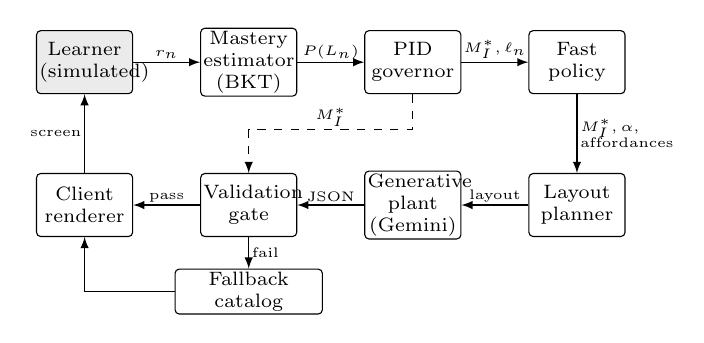
\begin{tikzpicture}[
  font=\scriptsize, >=latex, node distance=5mm and 8.5mm,
  box/.style={draw, rounded corners=1.5pt, align=center, minimum height=8mm, text width=11.5mm, inner sep=1pt},
  ext/.style={box, fill=black!8},
  lab/.style={font=\tiny, inner sep=1pt}]
\node[ext] (learner) {Learner\\(simulated)};
\node[box, right=of learner] (bkt) {Mastery\\estimator\\(BKT)};
\node[box, right=of bkt] (pid) {PID\\governor};
\node[box, right=of pid] (pol) {Fast\\policy};
\node[box, below=10mm of pol] (plan) {Layout\\planner};
\node[box, left=of plan] (plant) {Generative\\plant\\(Gemini)};
\node[box, left=of plant] (gate) {Validation\\gate};
\node[box, left=of gate] (render) {Client\\renderer};
\node[box, below=4mm of gate, text width=18mm, minimum height=5.5mm] (fb) {Fallback catalog};
\draw[->] (learner) -- node[lab, above]{$r_n$} (bkt);
\draw[->] (bkt) -- node[lab, above]{$P(L_n)$} (pid);
\draw[->] (pid) -- node[lab, above]{$M_I^*,\ell_n$} (pol);
\draw[->] (pol) -- node[lab, right, align=left]{$M_I^*,\alpha$,\\affordances} (plan);
\draw[->] (plan) -- node[lab, above]{layout} (plant);
\draw[->] (plant) -- node[lab, above]{JSON} (gate);
\draw[->] (gate) -- node[lab, above]{pass} (render);
\draw[->] (gate) -- node[lab, right]{fail} (fb);
\draw[->] (fb) -| (render);
\draw[->] (render) -- node[lab, left]{screen} (learner);
\draw[->, dashed] (pid.south) -- ++(0,-4.5mm) -| node[lab, pos=0.25, above]{$M_I^*$} (gate.north);
\end{tikzpicture}
}
\caption{The closed loop as deployed. The gate rechecks the budget
(dashed); failing trees are replaced from the fallback catalog. The learner
(shaded) is simulated here.}
\label{fig:arch}
\end{figure}

The loop has five stages (Fig.~\ref{fig:arch}): a psychometric
estimator, a complexity governor, a fast policy, a layout planner, and a
generative plant whose output passes a validation gate before a
deterministic client renders it.

\subsection{Mastery estimation}
After response $r_n\in\{0,1\}$ the mastery estimate is updated by Bayes' rule
and the learning transition \cite{corbett1995knowledge}. Writing
$p=P(L_n)$, $g=P(G)$, $s=P(S)$ and $\hat p=P(L_n\mid r_n)$,
\begin{align}
P(L_n\mid r_n{=}1) &= \frac{p(1-s)}{p(1-s) + (1-p)g},\\
P(L_n\mid r_n{=}0) &= \frac{ps}{ps + (1-p)(1-g)},\\
P(L_{n+1}) &= \hat p\,(1-P(F)) + (1-\hat p)\,P(T),
\end{align}
where $P(F)=0$ gives standard BKT and $P(F)>0$ adds forgetting
\cite{khajah2016deep}. Default parameters are $P(L_0)=0.15$, $P(T)=0.12$,
$P(G)=0.20$, $P(S)=0.08$. They are design values, not fitted (sensitivity in Section~\ref{sec:sensitivity}); they satisfy
the bounds $P(G)<0.3$, $P(S)<0.1$ \cite{corbett1995knowledge} and the
non-degeneracy conditions $P(G)+P(S)<1$, $P(T)<1-P(S)/(1-P(G))$
\cite{vandesande2013properties}.

\subsection{Complexity governor}
The setpoint is the conventional mastery threshold $P^*=0.95$
\cite{corbett1995knowledge,zhang2025mastery}. The tracking error is normalized
on each side of the setpoint so that deficit and surplus have equal
authority:
\begin{equation}
e_n=\begin{cases}(P^*-P(L_n))/P^* & P(L_n)\le P^*\\
(P^*-P(L_n))/(1-P^*) & P(L_n)>P^*\end{cases}
\end{equation}
so that $e_n\in[-1,1]$.
The control effort is
\begin{equation}
u_n = K_p e_n + K_i S_n + K_d D_n,
\end{equation}
with the clamped integral $S_n=\mathrm{clamp}(S_{n-1}+e_n,\,-S_{\max},\,S_{\max})$
for anti-windup \cite{astrom1989windup} and the first-order filtered derivative
$D_n=\gamma(e_n-e_{n-1})+(1-\gamma)D_{n-1}$ \cite{astrom2006advanced}. An
inverted logistic maps effort to the complexity budget,
\begin{equation}
M_I^* = \bigl(1+e^{k u_n}\bigr)^{-1},
\end{equation}
which is quantized into four levels $\ell_n=\min(4,1+\lfloor 4M_I^*\rfloor)$. A
hysteresis deadband $\Delta_h$ commits a new budget only when it differs from
the last committed budget by at least $\Delta_h$. The governor steps once per
response (unit sample time) from $S_0=D_0=0$ with $e_{-1}=e_0$, so the first
step has no derivative kick, and its first budget is always committed.

\paragraph*{Gain selection}
Classical tuning rules \cite{ziegler1942optimum,skogestad2003simple}
assume an identified plant, but here the interface does not alter simulated
responses (Section~\ref{sec:method}). Instead, $K_p$, $K_i$, $K_d$, $\gamma$,
$S_{\max}$ and $\Delta_h$ were selected by minimizing the cost $\mathrm{ITAE}+J$
(Section~\ref{sec:method}) \cite{graham1953itae} on a separate 1,000-learner
tuning cohort; all reported results use a disjoint test cohort. A random search
of 200 uniform samples over $K_p\in[0.25,2.5]$, $K_i\in[0,0.4]$, $K_d,\gamma\in
[0,1]$ ($\gamma\ge 0.05$), $S_{\max}\in[1,6]$, $\Delta_h\in[0.02,0.15]$ selected
$K_p=0.865$, $K_i=0.377$, $K_d=0.672$, $\gamma=0.398$, $S_{\max}=1.253$ and
$\Delta_h=0.141$. The cost surface is flat: the selected point scores 0.104
on the tuning cohort against 0.110 for hand-set initial values, which rank
22nd of 201. The logistic slope is $k=\ln 19/(K_p+K_iS_{\max})=2.202$, so
that the effort range $\pm(K_p+K_iS_{\max})$ maps to $[0.05,0.95]$.

\subsection{Fast policy}
A fast policy maps $(P(L_n), M_I^*, \ell_n, \text{recent errors})$ to discrete
affordances: scaffolding mode (worked example, guided scaffold, open
symbolic), whether to show the balance-scale manipulative, whether hints are
enabled, and an instructional density limit. The policy is deterministic
and rule-based in every reported result. An open-weight decision model
\cite{laya2026}, evaluated zero-shot, took 1.32\,s per decision (median, CPU)
and chose a worked example in all 200 test states, so it is not used.

\subsection{Layout planner, generative plant and validation gate}
The planner turns the budget into a layout. The policy fixes the abstraction
level $\alpha$; the planner then enumerates every admissible layout with
1--8 interactive elements, 0--3 hint tiers and nesting depth 1--4 (at most
102 valid layouts) and picks the one whose $M_I$ is closest to $M_I^*$. It keeps a requested worked
example when that stays within $\varepsilon$; ties go to fewer elements,
then shallower nesting. The plant, Gemini 3.7 Flash served
through Vertex AI, receives this layout with the policy decision and the
equation and writes the content as a JSON component tree. In the original
design (\emph{free} mode) the plant also chose the layout; we measure both
(Table~\ref{tab:gemini}). Nodes are
drawn from a closed set of six components (balance scale, worked step,
operation pad, symbolic workspace, hint accordion, verification plane). The client renders these components
directly and never executes generated code. Each emission is parsed against
the schema; if parsing fails, or if
$|M_I-M_I^*|>\varepsilon$ with $\varepsilon=0.05$, a precompiled fallback
tree is rendered instead: the planner's layout for the nearest of 41 budgets
1/40 apart, within $\varepsilon$ for every budget and policy decision (worst 0.049). A web client renders the
trees for inspection (Fig.~\ref{fig:screens}); the benchmark does not use it.

\begin{figure*}[t]
\centering
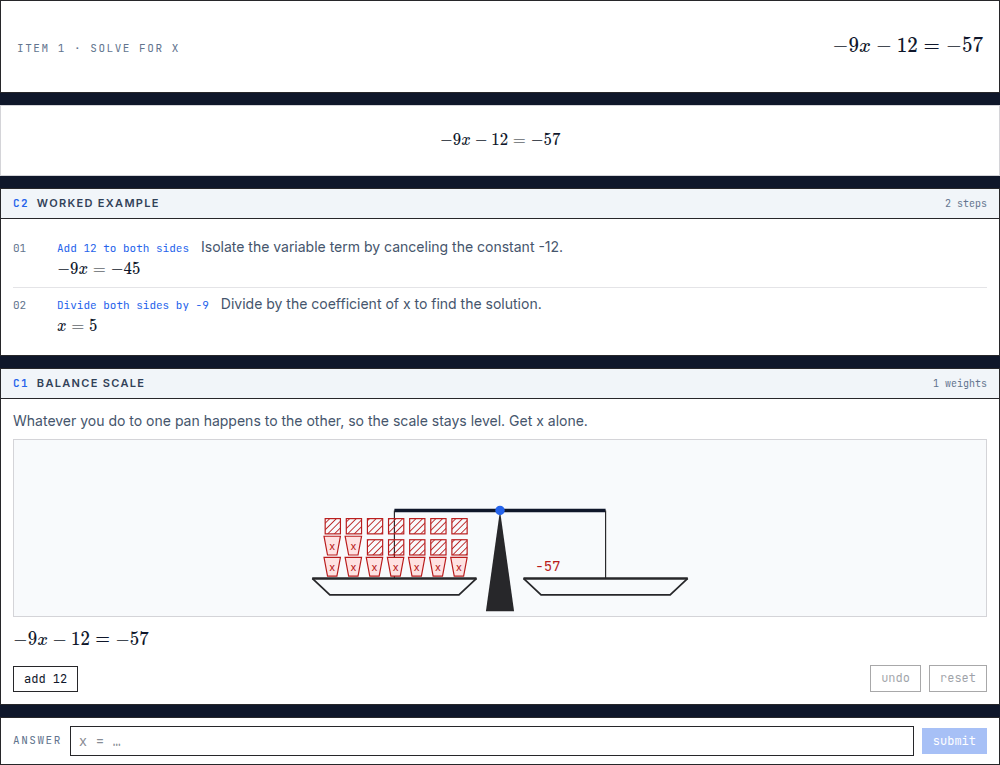
\includegraphics[height=3.5cm]{figures/screen_l1.png}\hspace{4mm}%
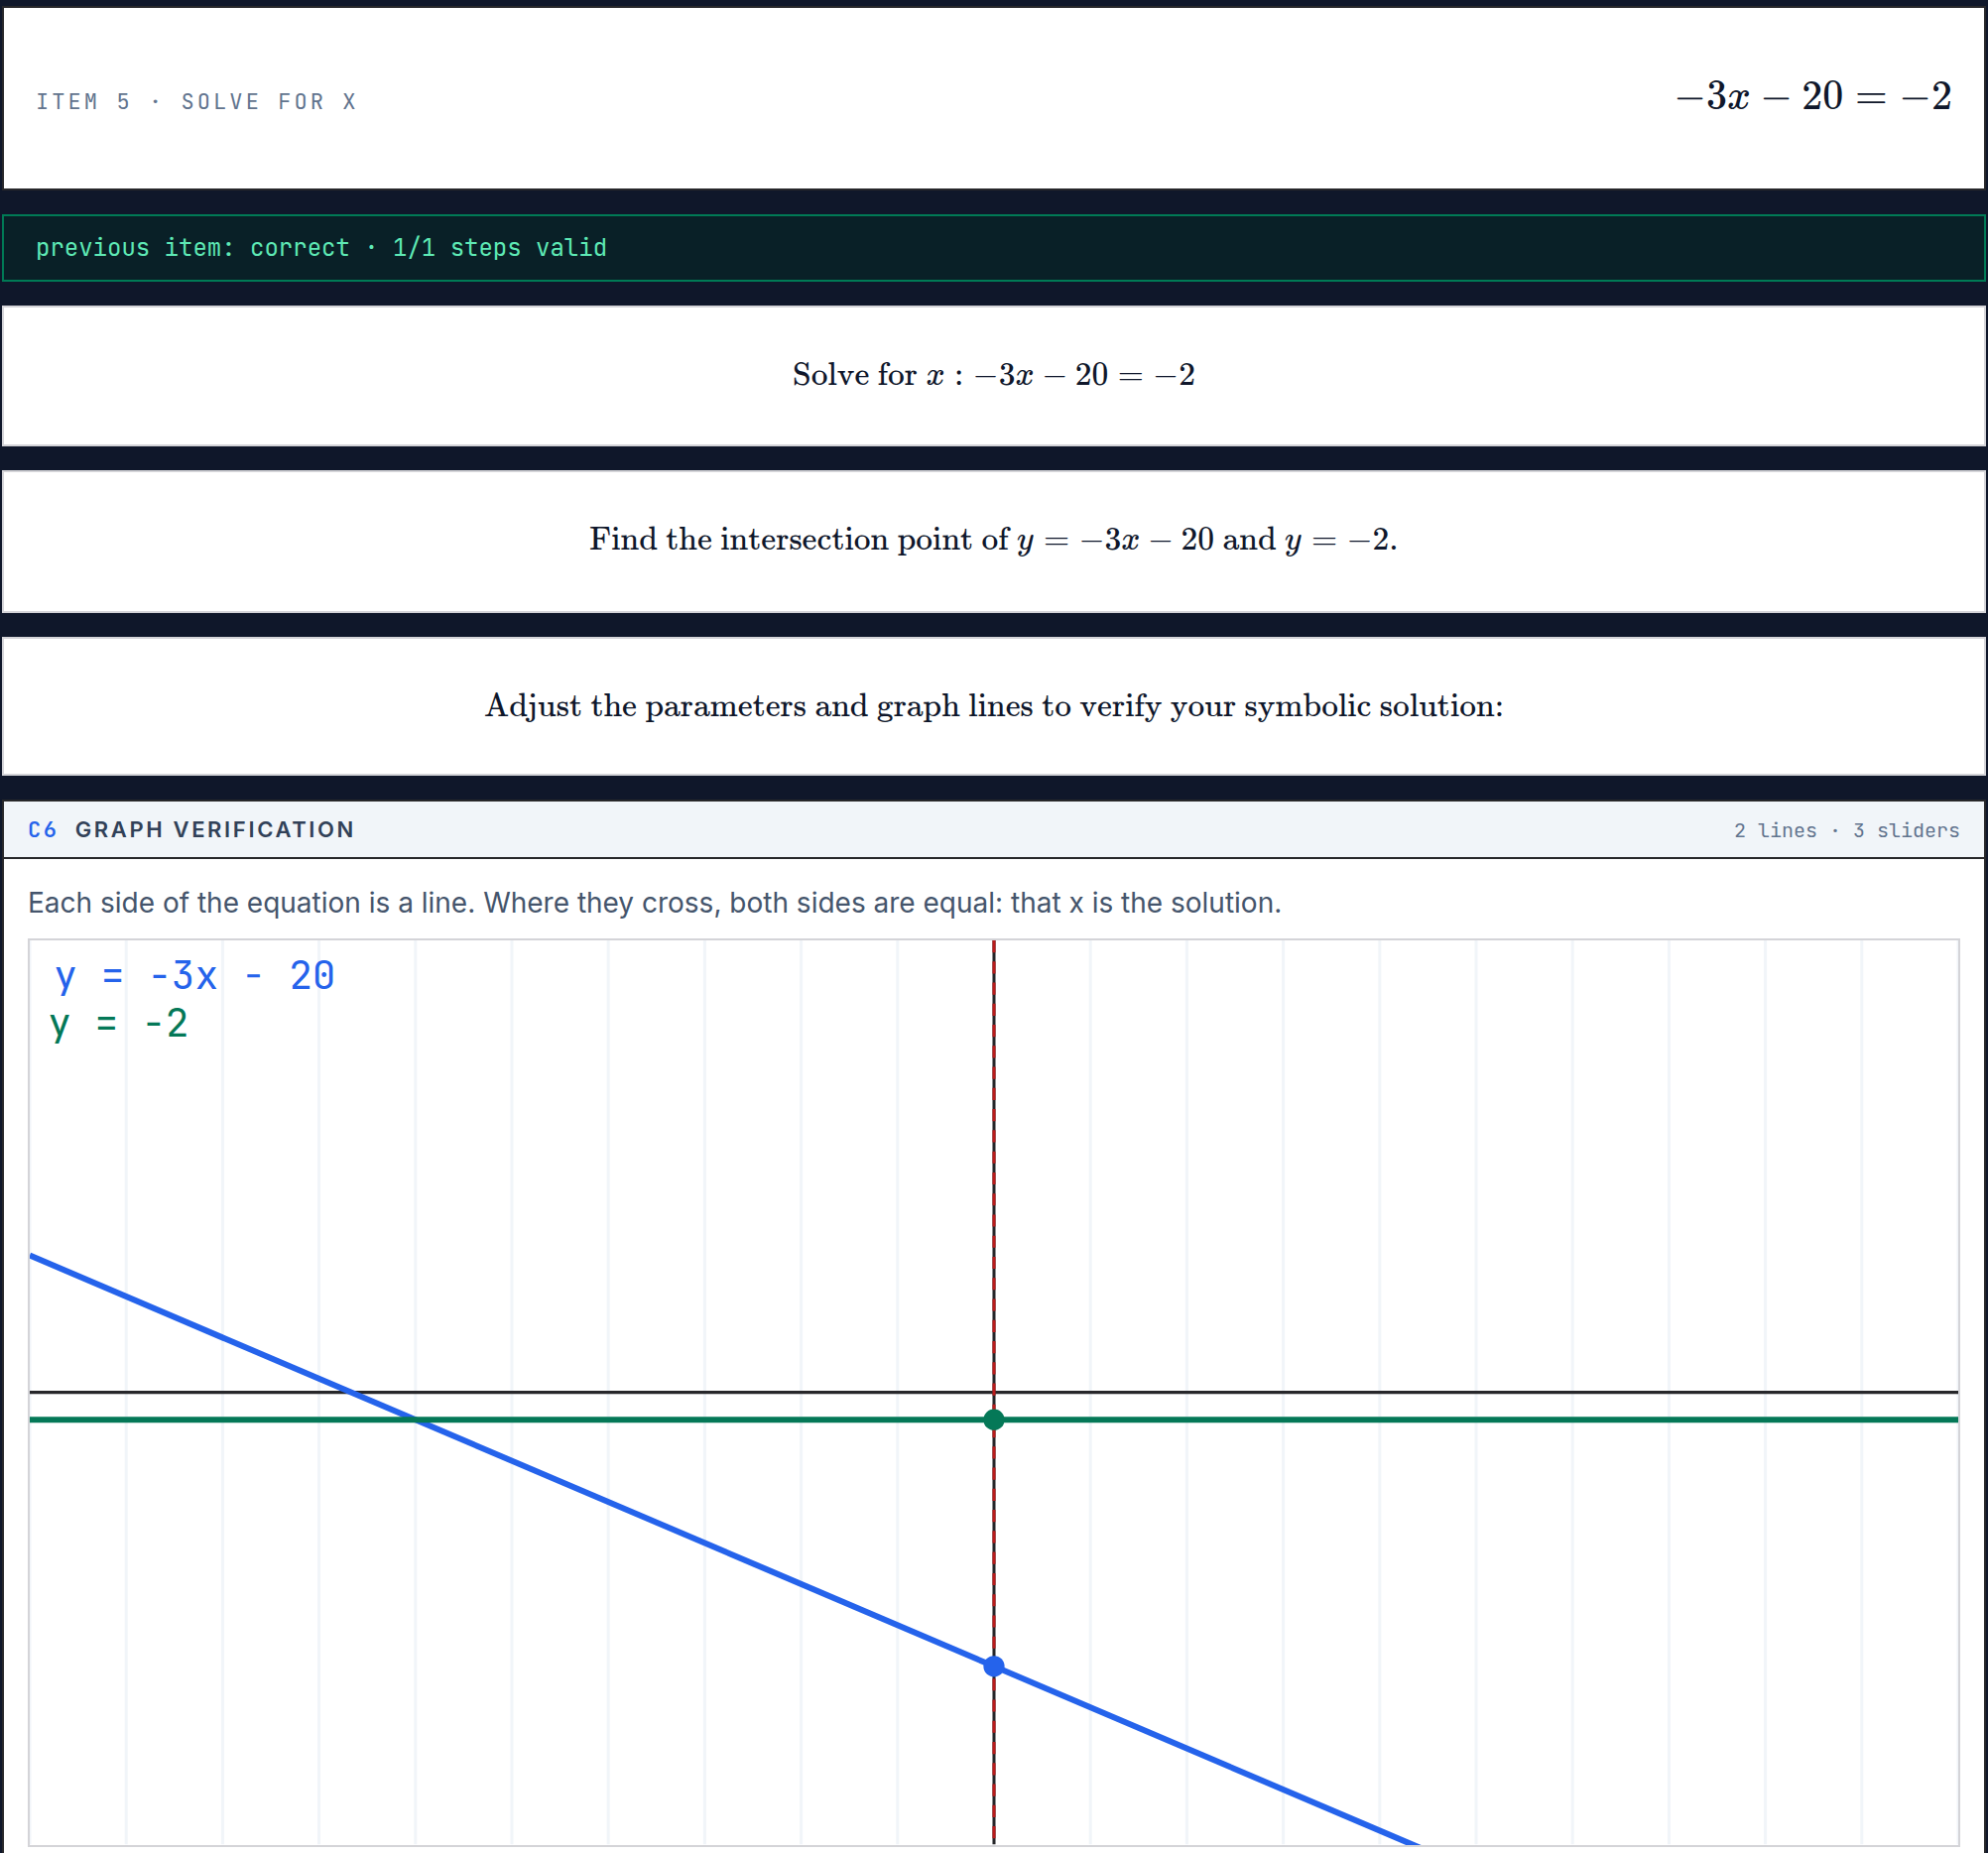
\includegraphics[height=3.5cm]{figures/screen_l4.png}
\caption{Screens written by Gemini 3.7 Flash in guided mode; both passed the
gate. Left: level 1, balance scale with a worked step ($M_I^*=0.091$,
$M_I=0.111$). Right: level 4, graph verification ($M_I^*=0.903$, $M_I=0.905$).}
\label{fig:screens}
\end{figure*}

\subsection{Structural complexity metric}
For a tree with $\rho$ interactive elements, abstraction level $\alpha$ and
nesting depth $\delta$,
\begin{equation}
M_I = w_1\frac{\rho-1}{7} + w_2\frac{\alpha-1}{3} + w_3\frac{\delta-1}{3},
\end{equation}
with $\rho\in[1,8]$ and $\alpha,\delta\in[1,4]$.
Each feature has a basis in prior work: element interactivity raises load \cite{sweller2010element}
and display density is a classic complexity measure \cite{tullis1983formatting};
the abstraction ladder from balance scale to operation pad to symbolic
workspace follows concreteness fading \cite{fyfe2014concreteness}; and
deeper structures cost users more \cite{kiger1984depth}.
Placing the Cartesian plane at the top of the ladder is our design choice.
With no data to fit weights, we use equal weights $w_i=1/3$, which are robust
in that setting \cite{dawes1979robust}, and test sensitivity to the weights
(Section~\ref{sec:results}). Entropy measures such as XAOS \cite{stickel2010xaos} score
rendered screens; $M_I$ scores the tree before rendering, as the gate requires.

% ---------------------------------------------------------------------------
\section{Method}
\label{sec:method}

\subsection{Synthetic learners}
Simulated learners are an established way to test instructional designs
before human studies \cite{vanlehn1994simulated,kaser2024simulated}, and
BKT-generated data have been used to evaluate mastery assessment
\cite{fancsali2013optimal}. Each learner is a two-state
HMM whose parameters are drawn uniformly from archetype ranges
(Table~\ref{tab:archetypes}). Novice and guesser ranges exceed the bounds
of \cite{corbett1995knowledge} by design but respect
\cite{vandesande2013properties}. The cohort has 1,000 learners
(300/400/300) with 40 items each. Responses are sampled once per learner and
replayed unchanged through every arm (paired design). The interface therefore
does not influence the simulated responses: the benchmark measures controller
behavior, not learning.

\begin{table}[t]
\centering
\caption{Learner archetypes (uniform parameter ranges).}
\label{tab:archetypes}
\begin{tabular}{lcccc}
\toprule
Archetype & $P(L_0)$ & $P(T)$ & $P(G)$ & $P(S)$\\
\midrule
Struggling novice & .02--.08 & .03--.07 & .10--.20 & .20--.30\\
Inconsistent guesser & .05--.20 & .10--.20 & .15--.40 & .08--.30\\
Fast master & .15--.30 & .30--.40 & .15--.25 & .01--.03\\
\bottomrule
\end{tabular}
\end{table}

\paragraph*{Arms}
All arms see the same responses and BKT estimate. (1) \emph{Static}: a fixed
level-2 interface. (2) \emph{Unconstrained GenUI}: the plant sets its own
complexity to the estimate plus Gaussian noise ($\sigma=0.15$); only the schema
is checked. (3) \emph{Rule-based}: step up after three consecutive correct
responses and down after two consecutive errors, an up-down rule in the
spirit of \cite{levitt1971updown}. Arms 1 and 3 render catalog trees. (4) \emph{Closed loop}:
the full architecture. Ablations remove the derivative filter, remove
anti-windup, and add a one-level slew limit.

\paragraph*{Plant model in the benchmark}
The benchmark replaces the foundation model with a surrogate that compiles
the planner's layout and injects faults: with probability 0.15 it
drifts off budget, and with probability 0.03 it emits malformed output
(e.g., truncated JSON, unknown component). These rates were set before the real model was measured.
The unconstrained arm uses the same surrogate without the budget check.

We measured the real model in free mode, which tests the model alone, and
in guided mode, the deployed configuration with the planner. Each mode received 300 requests (JSON mode without a response
schema, thinking level low, temperature 0.4, 30\,s timeout) with budgets
uniform on $[0.02,0.98]$, scored by the same gate (Table~\ref{tab:gemini}).

\begin{table}[t]
\centering
\caption{Gemini 3.7 Flash, 300 calls per mode.}
\label{tab:gemini}
\begin{tabular}{lcc}
\toprule
 & Free & Guided\\
\midrule
Transport failures (HTTP error, timeout) & 6 & 4\\
Content-malformed, of completed calls & 3.4\% & 0\%\\
Off budget, of valid trees & 2.8\% & 0\%\\
Raw output within budget, of all calls & 92.0\% & 98.7\%\\
Median $|M_I-M_I^*|$ of valid trees & 0.012 & 0.007\\
Latency of completed calls, median / p95 & 7.7 / 18.6\,s & 2.7 / 5.1\,s\\
\bottomrule
\end{tabular}
\end{table}

Free-mode failures lacked an interactive element (10/294) or missed the
budget (8/284, mostly level 1); guided-mode failures were all in transport. The surrogate's 3\% malformed
rate thus matches free mode, and its 15\% drift rate is a stress setting.
Compliance counts raw outputs over all calls; after the gate, every
rendered tree met the budget.

\paragraph*{Metrics}
Constraint error $\Delta M=|M_I-M^*_{\mathrm{ref}}|$ is measured against the
budget the closed-loop governor commits for the same responses, so that all
arms share one reference; ``within $\varepsilon$'' is the share of steps with
$\Delta M\le 0.05$. Interface jitter is
$J=\frac{1}{N-1}\sum_n|M_I(n)-M_I(n-1)|$, and a skip is a change of two or
more levels between consecutive items. Jitter operationalizes the
stability concern of \cite{gajos2008predictability}; the formula is ours.
Recovery time is the number of items after a streak of five or more errors
until the level returns to its pre-streak value. Fallback rate is the share
of steps rendered from the fallback catalog. Because the simulator knows the
learner's latent state, we also report \emph{overload} (level 3 or 4 shown
while the skill is not known), \emph{underload} (level 1 or 2 shown while it
is known) and an ITAE-weighted mismatch $\sum_n (n{+}1)m_n/\sum_n(n{+}1)$
\cite{graham1953itae}, where $m_n$ marks either case. These are level
mismatches, not measured load.

% ---------------------------------------------------------------------------
\section{Results}
\label{sec:results}

All numbers come from one run on the test cohort (seed 20261003; tuning
seed 20261004), with normal-approximation 95\% CIs over 1,000 learners. The CIs reflect
variation across learners in this run. Over ten independent test seeds the
ranking of arms never changed and the closed loop's $\Delta M$ stayed within 0.0118--0.0122.

\begin{table*}[t]
\centering
\caption{Main results and ablations on the test cohort.
$\Delta M$ and ``within $\varepsilon$'' are measured against the closed-loop
reference budget; every closed-loop variant meets its own budget at every step. Overload,
underload and ITAE use the latent learner state and exist only in simulation.
Fallback rates follow from the surrogate's fault rates.}
\label{tab:main}
\begin{tabular}{lcccccccc}
\toprule
Arm & $\Delta M$ (95\% CI) & Within $\varepsilon$ & Jitter $J$ & Skips/run & Overload & Underload & ITAE & Fallback\\
\midrule
Static & 0.426 (0.422--0.430) & 0.004 & 0.000 & 0.00 & 0.000 & 0.800 & 0.892 & --\\
Unconstrained GenUI & 0.131 (0.128--0.134) & 0.321 & 0.123 & 2.06 & 0.024 & 0.054 & 0.043 & 0.030\\
Rule-based & 0.123 (0.119--0.128) & 0.596 & 0.025 & 0.00 & 0.000 & 0.245 & 0.180 & --\\
Closed loop & 0.0122 (0.0119--0.0124) & 1.000 & 0.035 & 0.67 & 0.002 & 0.121 & 0.073 & 0.154\\
\midrule
\quad no derivative filter & 0.031 (0.030--0.033) & 0.811 & 0.044 & 1.19 & 0.002 & 0.124 & 0.076 & 0.156\\
\quad no anti-windup & 0.107 (0.102--0.112) & 0.549 & 0.024 & 0.42 & 0.001 & 0.217 & 0.174 & 0.159\\
\quad one-level slew limit & 0.025 (0.023--0.026) & 0.875 & 0.034 & 0.02 & 0.002 & 0.121 & 0.073 & 0.153\\
\bottomrule
\end{tabular}
\end{table*}

\begin{figure}[t]
\centering
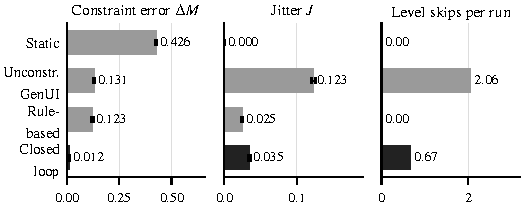
\includegraphics[width=\columnwidth]{figures/results.pdf}
\caption{Main comparison on the test cohort (means, 95\% CIs); closed loop
dark.}
\label{fig:results}
\end{figure}

\subsection{Main comparison}
The closed loop keeps the rendered interface within 0.012 of its budget
on average (Table~\ref{tab:main}, Fig.~\ref{fig:results}), against 0.131
and 0.123 for unconstrained GenUI and the rule-based arm. Every rendered tree
is within $\varepsilon$, partly by construction: the generator's own output met
the budget on 84.6\% of steps, and the gate replaced the other 15.4\% from the
fallback catalog. The closed loop's jitter (0.035) is 3.5 times lower than that of
unconstrained GenUI (0.123), which also skips levels 2.06 times per run
against 0.67. The rule-based arm is smoother still (0.025, no skips), because
it moves one level at a time. Against the latent learner state, the picture
is mixed. Unconstrained GenUI has the lowest ITAE mismatch (0.043 against
0.073) and the least underload (5.4\% of steps against 12.1\%), but shows an
abstract interface to a learner who does not know the skill twelve times as
often (2.4\% against 0.2\%). After streaks of five or more errors that lowered the level, the closed
loop regained its pre-streak level in 34 of 51 cases (median 5 items), the
rule-based arm in 9 of 19 (median 12).

\subsection{Ablations}
Removing the derivative filter raises jitter from 0.035 to 0.044 and nearly
doubles level skips (1.19 per run). Removing anti-windup lets the integral
grow without bound: underload rises from 12.1\% to 21.7\%, only 84\% of
learners reach level 4 against 95\%, and median recovery after an error
streak grows from 5 to 14 items. A one-level slew limit removes nearly all skips (0.02 per
run) and leaves the ground-truth measures unchanged.

\subsection{Sensitivity}
\label{sec:sensitivity}
Changing each controller parameter by $\pm 50\%$ raised the cost
($\mathrm{ITAE}+J$) from 0.108 to at most 0.118, except $1.5\Delta_h$,
which lowered it to 0.104 but more than doubled level skips. For the
metric weights, the closed loop's $\Delta M$ stays between 0.007 and 0.017
under equal weights, the initial $0.40/0.35/0.25$ split and three
single-feature-heavy splits ($0.6/0.2/0.2$). Dropping abstraction or depth
roughly doubles it (0.023 and 0.022) while keeping more than 99\% of steps
within $\varepsilon$. Dropping element density breaks the loop: fallbacks rise to 84\% and only
18\% of screens are within $\varepsilon$. Changing each BKT parameter by
$\pm 50\%$ kept every step within $\varepsilon$, $\Delta M$ between 0.010 and
0.017, jitter between 0.034 and 0.041 and fallbacks at 15--16\%. The
parameters mainly shift when the interface escalates: $P(T)$ and $P(G)$ move
ITAE between 0.048 and 0.115, and skips rise to at most 1.20 per run.

\subsection{BKT saturation and lapse handling}
Under correct responses the BKT estimate converges to a stable fixed point at
one \cite{vandesande2013properties}. With the default parameters the estimate
exceeds $1-10^{-6}$ after ten correct responses and five subsequent errors
lower it only to about $0.98$; after 24 correct responses it
equals $1.0$ in double precision and no further evidence can lower it.  The interface
then stays at its highest level through a streak of errors.
We compare two remedies: forgetting, $P(F)>0$ \cite{khajah2016deep},
and a CUSUM detector \cite{page1954cusum} on the
log-likelihood ratio between ``not known'' and the tracker's prediction,
which resets the estimate to 0.5 when the sum exceeds $h=6.5$. It
accumulates only when a confident estimate is contradicted, so isolated
slips are absorbed; unlike neural forgetting models, it needs no training data. Forgetting uses $P(F)=0.02$.

\begin{figure}[t]
\centering
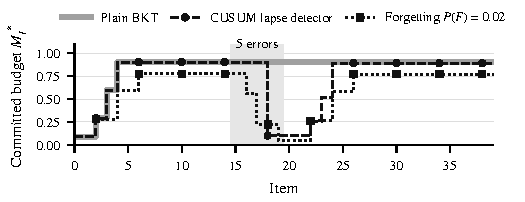
\includegraphics[width=\columnwidth]{figures/probe.pdf}
\caption{Scripted probe: 15 correct responses, five errors, then correct
again. With plain BKT the estimate is saturated and the budget never moves.}
\label{fig:probe}
\end{figure}

In a scripted probe with fifteen correct responses followed by five errors
(Fig.~\ref{fig:probe}), the plain closed loop never lowers the interface; the CUSUM variant drops a
level 3 items after the streak begins and forgetting after 1. To test this
at scale, a second cohort of 1,000 learners can forget the skill with
probability 0.02--0.06 per item. There the plain closed loop shows an
abstract interface to a learner who does not know the skill on 7.6\% of
steps. The CUSUM detector lowers this to 5.6\% ($-25\%$) at the cost of
higher jitter (0.052 against 0.042) and an almost unchanged ITAE mismatch
(0.189 against 0.184). Forgetting lowers overload further, to 3.0\%, but
underloads on 25.3\% of steps against 12.8\%, raises ITAE to 0.273 and
lets only 80\% of learners reach level 4. Neither remedy dominates; weighting recent responses
\cite{galyardt2015recent} is left for future work.

% ---------------------------------------------------------------------------
\section{Discussion and Limitations}

The benchmark tests whether the controller does what it is designed to do; it
does not test whether learners benefit. Because simulated responses do not
depend on the interface, the loop is closed only through the mastery
estimate, not through the learner. $M_I$ is a structural proxy that has not
been validated against measured or perceived load, for which instruments
exist \cite{leppink2013instrument}; the results show structural complexity
regulation, not reduced cognitive load. BKT
parameters are design values rather than fits to tutor data. Long error
streaks may reflect misconceptions rather than slips
\cite{booth2014persistent}; the controller does not distinguish these.
The real model was measured on single calls, not full trajectories. Its latency (median 7.7\,s free,
2.7\,s guided) calls for prefetching or caching. We tested one domain, linear equations.

\section{Conclusion}
We coupled a learner model to a generative interface through a PID
governor, a layout planner and a validation gate, and tested the loop in
simulation. The governor's budget is met at every step, with the gate
replacing the 15.4\% of generated trees that miss it, and the interface changes 3.5 times less than an
unconstrained generator while rarely showing abstract screens to simulated
learners who have not mastered the skill. Anti-windup and the derivative filter each
matter, and a slew limit removes level skips. A CUSUM lapse detector restores
BKT's reaction after long success runs at a modest cost in jitter. In 300 single real calls, 98.7\% of
raw outputs met the budget with the planner and 92\% without it. Next steps are full
real-model trajectories, a learned fast policy and a study with learners. We claim
structural budget regulation in simulation, not learning gains or reduced
cognitive load.

\section*{Code and Data Availability}
The engine, simulation harness, benchmark results and the sources of
this manuscript are openly available at \url{https://github.com/omanandswami2005/closed-loop-genui-research-implementation}.

\bibliographystyle{IEEEtran}
\bibliography{../docs/references}

\end{document}
